\chapter{Reti di Petri}
Abbiamo introdotto un'algebra di processi come CCS dove processi sequenziali
interagiscono tra loro tramite hand-shaking. Un altro modello usato, con varie
implementazioni, sono gli automi a stati finiti. Si passa ora alle reti di Petri.

La critica di Petri è che in un sistema distribuito non sia individuabile uno
stato globale, che in un sistema distribuito le trasformazioni di stato siano
localizzate e non globali, che non esista un sistema di riferimento temporale
unico. Quindi la simulazione sequenziale non deterministica (semantica a
“interleaving”) dei sistemi distribuiti è una forzatura e non rappresenta le
reali caratteristiche del comportamento del sistema, ovvero la località, la
distribuzione degli eventi e la relazione di dipendenza causale e non causale
tra gli eventi.

Nel modello proposto da Petri, le azioni vengono rappresentate come nodi
dell'automa e non più come etichette della transizione. Oltre a ciò, le azioni e
le coazioni che abbiamo definito in CCS per sincronizzare due processi diventano
una singola azione di sincronizzazione.

Petri sviluppò una teoria matematica fondata sui principi della fisica moderna,
che sia una teoria dei sistemi in grado di descrivere il flusso di informazione
e permetta di analizzare sistemi con organizzazione complessa.

Lo \textbf{stato} è definito da una collezione di stati locali.
\section{Reti elementari}
\begin{definizione}[\textbf{Rete}]
    Una \textbf{rete} è definite come:
    \begin{equation}
        N = (B, E, F)
    \end{equation}
    dove:
    \begin{itemize}
        \item $B$ è un insieme finito di condizioni, anche detti stati locali,
              proposizioni vere o false. Rappresentato da: $$\bigcirc$$
        \item $E$ è un insieme finito di eventi, \textbf{trasformazioni locali}
              di stato. Rappresentato da: $$\Box$$
              \begin{equation}
                  B\cap E  = \emptyset \land B\cup E \ne \emptyset
              \end{equation}
        \item $F \subseteq (B \times E) \cup (E \times B)$ è una
              \textbf{relazione di flusso} Rappresentato da: $$\to$$
              Inoltre, la relazione di flusso è tale per cui non esistano elementi
              isolati, in quanto non avrebbero senso. Si ha, formalmente, che:
              \begin{equation}
                  dom(F) \cup ran(F) = B \cup E
              \end{equation}
              ovvero non ho condizioni/eventi isolati, in quanto non avrebbero
              senso, avrei una condizione costante e un evento che non accade
              mai; quindi, dominio e codominio di $F$ coprono l'insieme di
              condizioni ed eventi.
    \end{itemize}
\end{definizione}
Sia $x \in X$ dove l'insieme $X$ è definito come $X = B \cup E$, allora possiamo
definire:
\begin{itemize}
    \item $^{\bullet} x =\{y \in X: \ (y, x) \in F\}$ sono i \textbf{pre-elementi}
          di $x$. Posso anche definirli come precondizioni o pre-eventi.
    \item $x^{\bullet} =\{y \in X: \ (x, y) \in F\}$ sono i \textbf{post-elementi}
          di $x$. Posso anche definirli come post-condizioni o post eventi.
\end{itemize}
Sia $A \subseteq B \cup E$ allora posso definire:
\begin{itemize}
    \item $^{\bullet} A = \bigcup_{x \in A} \ ^{\bullet} x$
    \item $A^{\bullet} = \bigcup_{x \in A} x^{\bullet}$
\end{itemize}
Nelle reti c'è sempre una relazione di dualità tra due elementi, per esempio tra
condizioni ed eventi, tra pre-eventi e post-eventi, tra precondizioni e post
condizioni. Inoltre, si ha la caratteristica della località, quindi si hanno stati
locali e trasformazioni di stato locali.

La rete $N = (B, E, F)$ descrive la struttura statica del sistema, il
comportamento è definito attraverso le nozioni di caso e di regola di scatto o
regola di transizione.

Un \textbf{caso} o \textbf{configurazione} è un insieme di condizioni $c \subseteq B$
che rappresentano l'insieme di condizioni vere in una certa configurazione del
sistema, un insieme di stati locali che collettivamente individuano lo
\textit{stato globale} del sistema.
\begin{itemize}
    \item Condizione vera: $$\bigodot$$
    \item Condizione falsa: $$\bigcirc$$
\end{itemize}
\begin{definizione} [\textbf{Regola dello scatto}]
    Sia $N = (B, E, F)$ una rete elementare e $c \subseteq B$. L'evento $e \in E$
    è \textbf{abilitato}, ovvero può occorrere, in $c$, denotato $c[e >$, se e
    solo se:
    \begin{equation}
        ^{\bullet} e \subseteq c \ \land \ e^{\bullet} \cap c = \emptyset
    \end{equation}
    Se $c[e >$, allora quando $e$ occorrere in $c$ genera un nuovo caso $c'$,
    denotato $c[e > c'$:
    \begin{equation}
        c' = (c - ^{\bullet} e) \cup e^{\bullet}
    \end{equation}
\end{definizione}
In altre parole, un evento $e$ è abilitato se le sue precondizioni sono vere,
le post-condizioni false. Lo scatto di $e$ rende le precondizioni false e le
post-condizioni vere, le altre condizioni rimangono inalterate.

Le reti si basano sul \textbf{principio di estensionalità}, ovvero sul fatto che
il cambiamento di stato è locale:
\begin{center}
    \textit{Un evento è completamente caratterizzato dai cambiamenti che produce
        negli stati locali, tali cambiamenti sono indipendenti dalla particolare
        configurazione in cui l'evento occorre.}
\end{center}
\begin{definizione}[]
    Sia $N = (B, E, F)$ una \textbf{rete elementare}, si ha che:
    \begin{itemize}
        \item $N$ è \textbf{semplice} se e solo se:
              \begin{equation}
                  \forall x, y \in B \cup E, \ ^{\bullet} x = \ ^{\bullet} y \
                  \land \ x^{\bullet} = y^{\bullet} \Rightarrow x = y
              \end{equation}
        \item $N$ è \textbf{pura} se e solo se:
              \begin{equation}
                  \forall e \in E: \ ^{\bullet}e \cap e^{\bullet} = \emptyset
              \end{equation}
    \end{itemize}
\end{definizione}
\begin{definizione}
    Sia $N = (B, E, F)$ una rete elementare, $U \subseteq E$ e $c, c_1, c_2 \subseteq B$.
    \begin{itemize}
        \item $U$ è un \textbf{insieme di eventi indipendenti} se e solo se:
              \begin{equation}
                  \forall e_1, e_2 \in U: \ e_1 \neq e_2 \Rightarrow (^{\bullet}e_1
                  \cup e_1^{\bullet}) \cap (^{\bullet}e_2 \cup e_2^{\bullet}) = \emptyset
              \end{equation}
        \item $U$ è un \textbf{passo abilitato} (insieme di eventi concorrenti)
              in $c$ anche scritto come $c[U >$ se e solo se:
              \begin{equation}
                  U \ \text{insieme di eventi indipendenti} \ \land \ \forall e
                  \in U: \ c[e >
              \end{equation}
        \item $U$ è un \textbf{passo} da $c_1$ a $c_2$, anche scritto come
              $c_1[U > c_2$ se e solo se:
              \begin{equation}
                  c_1 [ U > \ \land \ c_2 = (c_1 - \ ^{\bullet} U) \cup U^{\bullet}
              \end{equation}
    \end{itemize}
    Se due eventi sono indipendenti allora possono eseguire in modo concorrente.
\end{definizione}
Un \textbf{sistema elementare} $\Sigma = (B, E, F; c_{in})$ è definito da una rete
$N = (B, E, F)$ e da $c_{in} \subseteq B$ un caso iniziale.
\begin{definizione}[\textbf{Caso raggiungibile}]
    L'insieme dei \textbf{casi raggiungibili} ($C_{\Sigma}$) del sistema elementare
    $\Sigma = (B, E, F; c_{in})$ è il più piccolo sottoinsieme di $2^B$ tale che:
    \begin{itemize}
        \item $c_{in} \in C_{\Sigma}$
        \item Se $c \in C_{\Sigma}, U \subseteq E, c' \subseteq B$ sono tali che:
              $c[U > c'$ allora $c' \in C_{\Sigma}$
    \end{itemize}
\end{definizione}
L'insieme $C_\Sigma$ è un insieme \textbf{finito} perché si parla di sottoinsiemi
di insiemi finiti che sono anch'essi finiti, ovviamente esplode in un esponenziale.
\begin{definizione}[\textbf{Insieme dei passi}]
    $U_{\Sigma}$ è l'\textbf{insieme dei passi} di $\Sigma$:
    \begin{equation}
        U_{\Sigma} = \{U \subseteq \ E | \exists c, c' \in C_{\Sigma}: c[U > c'\}
    \end{equation}
\end{definizione}
Sia $\Sigma = (B, E, F; c_{in})$ un sistema elementare,
$c_i \in C_{\Sigma}, e_i \in E, U_i \subseteq E$ possiamo distinguere:
\begin{itemize}
    \item \textbf{Comportamento sequenziale}: sequenze di occorrenze o di eventi
          (”interleaving”, simulazione sequenziale non deterministica), ovvero una
          sequenza di eventi che possono occorrere dal caso iniziale, facendo scattare
          in maniera sequenziale gli eventi uno alla volta in $c_n$:
          \begin{equation}
              c_{in}[e_1 > c_1[e_2 > \dots [e_n > c_n \ \text{oppure} \
              c_{in}[e_1e_2 \dots e_n > c_n
          \end{equation}
    \item \textbf{Comportamento non sequenziale} (semantica a passi): sequenze di
          passi (”step semantics”) in quanto possiamo anche considerare insiemi
          di eventi, ovvero passi:
          \begin{equation}
              c_{in}[U_1 > c_1[U_2 > \dots [U_n > c_n \ \text{oppure} \
              c_{in}[U_1U_2 \dots U_n > c_n
          \end{equation}
    \item \textbf{Comportamento non sequenziale}  (semantica di ordine parziale):
          processi non sequenziali (”partial order semantics” - ”true concurrency”).
          Il comportamento di tale sistema viene registrato in una rete di Petri.
\end{itemize}
Si considerano sia sequenze finite che sequenze infinite (di eventi o di passi).

Il comportamento di un sistema elementare $\Sigma = (B, E, F; c_{in})$ può essere
rappresentato dal suo grafo dei casi.
\begin{definizione}[\textbf{Grafo dei casi}]
    Il \textbf{grafo dei casi} di $\Sigma$ è il sistema di transizioni etichettato
    $CG_{\Sigma} = (C_{\Sigma},U_{\Sigma}, A, c_{in})$ dove:
    \begin{itemize}
        \item $C_{\Sigma}$ è l'insieme dei nodi del grafo (gli stati globali).
        \item $U_{\Sigma}$ è l'alfabeto.
        \item $A$ è l'insieme di archi etichettati:
              \begin{equation}
                  A = \{(c, U, c') | c, c' \in C_{\Sigma}, U \in U_{\Sigma}, c[U > c'\}
              \end{equation}
              I nodi sono i casi sequenziali mentre gli archi sono gli eventi
    \end{itemize}
\end{definizione}
\begin{definizione}[\textbf{Grafo dei casi sequenziale}]
    Il \textbf{grafo dei casi sequenziali} di $\Sigma=(B,E,F;c_{in})$ è
    il sistema di transizioni etichettato $SCG_\Sigma=(C_\Sigma, E, A,c_{in})$
    dove:
    \begin{equation}
        A=\left\{(c,e,c')|c,c'\in C_\Sigma, e\in E: c[e>c' \right\}
    \end{equation}
\end{definizione}
\subsection{Diamond property}
\begin{definizione} [\textbf{Diamond property}]
    Sia $\Sigma = (B, E, F; c_{in})$ un sistema elementare,
    $CG_{\Sigma} = (C_{\Sigma},U_{\Sigma}, A, c_{in})$ il suo grafi dei casi,
    $U_1,U_2 \in U_{\Sigma}: U_1 \cap U_2 = \emptyset, U_1 \neq \emptyset, U_2
        \neq \emptyset$, e $c_1, c_2, c_3, c_4 \in C_{\Sigma}$, allora valgono:
    \begin{enumerate}
        \item Dato $c_1[e_1 >$ e $c_1[e_2 >$ segue che:
              \begin{equation}
                  ^{\bullet}e_1 \cap e_2^{\bullet} = \emptyset \ \land \
                  ^{\bullet}e_2 \cap e_1^{\bullet} = \emptyset
              \end{equation}
              infatti, se $e_1$ e $e_2$ sono entrambi abilitati in $c_1$, le loro
              precondizioni sono vere e le post-condizioni false, e quindi non è
              possibile che una condizione sia contemporaneamente precondizione di
              $e_1$ (vera) e anche post-condizione di $e_2$ (falsa), e viceversa.

              Da $c_1[e_1 > c_2[e_2  >$ segue:
              \begin{equation}
                  ^{\bullet} e_1 \cap ^{\bullet} e_2 = \emptyset \ \land \
                  e_1^{\bullet} \cap e_2^{\bullet} = \emptyset
              \end{equation}
              in $c_2$, infatti, le precondizioni di $e_1$ sono false mentre le
              precondizioni di $e_2$ sono vere e quindi $e_1$ e $e_2$ non possono
              avere precondizioni in comune. Inoltre, sempre in $c_2$ le post-condizioni
              di $e_1$ sono vere, mentre quelle di $e_2$ sono false, e quindi
              $e_1$ e $e_2$ non possono avere post-condizioni in comune. Segue
              quindi \ref{fig:dp1}.
              \begin{figure}[!ht]
                  \centering
                  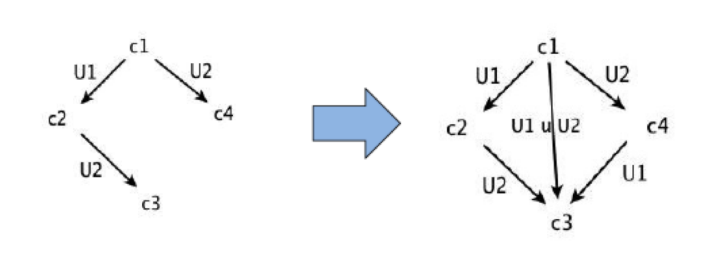
\includegraphics[width=0.5\textwidth]{img/reti/dp1.png}
                  \caption{Diamond property 1}
                  \label{fig:dp1}
              \end{figure}
        \item Supponiamo che $U_1 \cup U_2 \in U_{\Sigma}$ e che
              $U_1 \cap U_2 = \emptyset$, $U_1 \neq \emptyset, U_2 \neq \emptyset$.
              Allora se $c_1[U_1 \cup U_2 >c_3$ sicuramente $c_1[U_1 >$ e $c_1[U_2 >$
              e anche: $c_1[U_1 > c_2[U_2 >c_3$ e $c_1[U_2 > c_4[U_1 >c_3$. Segue
              quindi \ref{fig:dp2}.
              \begin{figure}[!ht]
                  \centering
                  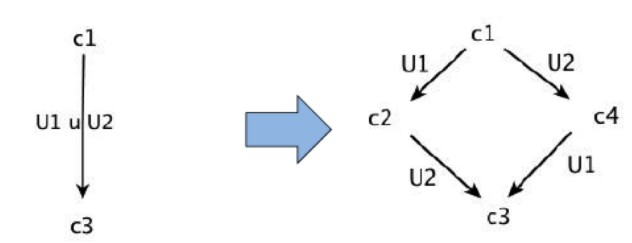
\includegraphics[width=0.5\textwidth]{img/reti/dp2.png}
                  \caption{Diamond property 2}
                  \label{fig:dp2}
              \end{figure}
    \end{enumerate}
\end{definizione}
Per la \textit{Diamond property}, nei sistemi elementari il grafo dei casi e il
grafo dei casi sequenziale sono \textit{sintatticamente equivalenti}, ovvero
possono essere ricavati l'uno dall'altro.

Questo implica il fatto che due sistemi elementari hanno grafi dei casi isomorfi
se e solo se hanno grafi dei casi sequenziale isomorfi.
\begin{definizione}[\textbf{Equivalenza tra sistemi}]
    Due sistemi $\Sigma_1$ e $\Sigma_2$ sono \textbf{equivalenti} se e solo se
    hanno grafi dei casi sequenziali, e quindi anche grafi dei casi, \textbf{isomorfi}.
\end{definizione}
\begin{definizione}[\textit{Problema della sintesi}]
    Dato un sistema di transizioni etichettato $A = (S, E,T,s_0)$, stabilire se
    esiste un sistema elementare $\Sigma = (B, E, F; c_{in})$ tale che: il suo
    grafo dei casi $SCG_{\Sigma}$ sia isomorfo ad $A$. E, in caso affermativo,
    costruire $\Sigma$.

    Questo problema è stato risolto usando la teoria delle regioni. Oltre a ciò,
    A dovrà soddisfare la Diamond property.
\end{definizione}
\begin{definizione}[\textbf{Contatto}]
    Sia $\Sigma = (B, E, F; c_{in})$ un sistema elementare, $e \in E$, $c \in
        C_{\Sigma}$ allora $(e, c)$ è un \textbf{contatto} se e solo se:
    \begin{equation}
        ^{\bullet}e \subseteq c \ \land \ e^{\bullet} \cap c \neq \emptyset
    \end{equation}
\end{definizione}
\begin{definizione}[\textbf{Sistema senza contatti}]
    Un sistema elementare $\Sigma = (B, E, F; c_{in})$ è \textbf{senza contatti}
    se e solo se:
    \begin{equation}
        \forall e \in E, \ \forall c \in C_{\Sigma} \ \text{si ha} \ ^{\bullet}e
        \subseteq c \Rightarrow e^{\bullet} \cap c = \emptyset
    \end{equation}
\end{definizione}
È possibile trasformare un sistema elementare $\Sigma$ con contatti in un
sistema elementare $\Sigma_0$ che sia senza contatti aggiungendo a $\Sigma$ il
complemento di ogni condizione si ottiene, un sistema $\Sigma_0$ con grafo dei
casi isomorfo a quello di $\Sigma$.
\begin{figure}[!ht]
    \centering
    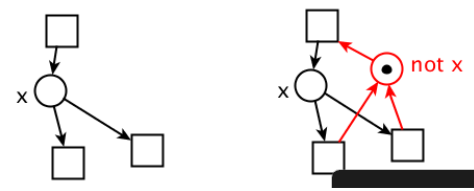
\includegraphics[width=0.5\textwidth]{img/reti/DelContatti.png}
    \caption{Complemento dell'operazione x.}
\end{figure}
Quindi se un sistema elementare $\Sigma$ è senza contatti allora per verificare
che un evento $e$ sia abilitato in un caso raggiungibile $c$ è sufficiente
verificare che le precondizioni di $e$ siano vere:
\begin{equation}
    c[e> \ \text{se e solo se} \ ^{\bullet} e \subseteq c
\end{equation}
\begin{definizione}[\textbf{Sequenza}]
    Sia $\Sigma = (B, E, F; c_{in})$ un sistema elementare, $c \in C_{\Sigma}$
    $e_1, e_2, \in E$, allora $e_1$ ed $e_2$ sono in \textbf{sequenza} in $c$
    se e solo se:
    \begin{equation}
        c[e_1 > \ \land \ \lnot c[e_2 > \ \land \ c[e_1e_2 > \ (c[e_1 > c'[e_2 >)
    \end{equation}
    \begin{figure}[!ht]
        \centering
        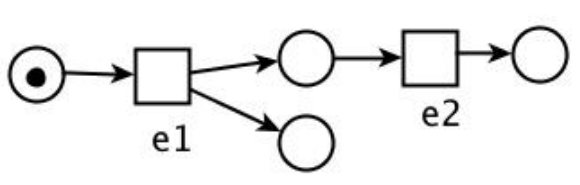
\includegraphics[width=0.5\textwidth]{img/reti/Seq.png}
        \caption{Rappresentazione della sequenza}
    \end{figure}
    In altre parole, è presente una relazione di dipendenza causale tra $e_1$ ed
    $e_2$.
\end{definizione}
\begin{definizione}[\textbf{Concorrenti}]
    Sia $\Sigma = (B, E, F; c_{in})$ un sistema elementare, $c \in C_{\Sigma}$
    $e_1, e_2, \in E$, allora $e_1$ ed $e_2$ sono \textbf{concorrenti} in $c$
    se e solo se:
    \begin{equation}
        c[\{e_1, e_2\} >
    \end{equation}
    \begin{figure}[!ht]
        \centering
        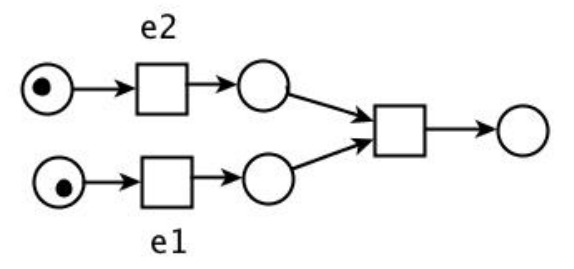
\includegraphics[width=0.5\textwidth]{img/reti/conc.png}
        \caption{Rappresentazione della concorrenza}
    \end{figure}
    In altre parole, se e sol se $e_1$ ed $e_2$ sono indipendenti ed entrambi
    abilitati in $c$.
\end{definizione}
\begin{definizione}[\textbf{Conflitto}]
    Sia $\Sigma = (B, E, F; c_{in})$ un sistema elementare,
    $c \in C_{\Sigma}$ $e_1, e_2, \in E$, allora $e_1$ ed $e_2$ sono in
    \textbf{conflitto} in $c$ se e solo se:
    \begin{equation}
        c[e_1 > \ \land \ c[e_2 > \ \land \ \lnot c[\{e_1, e_2\} >
    \end{equation}
    \begin{figure}[!ht]
        \centering
        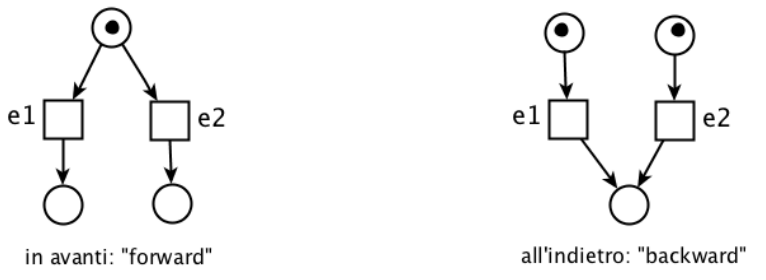
\includegraphics[width=0.5\textwidth]{img/reti/conf.png}
        \caption{Rappresentazione di un conflitto}
    \end{figure}
    In altre parole, sono entrambi abilitati ma l'occorrenza di uno disabilita
    l'altro.
\end{definizione}
Si definisce \textbf{confusione} quando non è possibile stabilire se è stato
risolto un conflitto.
\begin{definizione}[\textbf{Sottorete}]
    Siano $N = (B, E, F)$ e $N_1 = (B_1, E_1, F_1)$ due reti elementari. Diciamo che:
    \begin{itemize}
        \item $N_1 = (B_1, E_1, F_1)$ è \textbf{sottorete} di $N$ se e solo se:
              \begin{itemize}
                  \item $B_1 \subseteq B$
                  \item $E_1 \subseteq E$
                  \item $F_1 = F \cap [(B_1 \times E_1) \cup (E_1 \times B_1)]$
              \end{itemize}
        \item $N_1 = (B_1, E_1, F_1)$ è \textbf{sottorete generata da} $B_1$ se e solo se:
              \begin{itemize}
                  \item $B_1 \subseteq B$
                  \item $E_1 \subseteq ^{\bullet} B_1 \cup B_1^{\bullet}$
                  \item $F_1 = F \cap [(B_1 \times E_1) \cup (E_1 \times B_1)]$
              \end{itemize}
        \item $N_1 = (B_1, E_1, F_1)$ è \textbf{sottorete generata da} $E_1$ se e solo se:
              \begin{itemize}
                  \item $B_1 \subseteq ^{\bullet} E_1 \cup E_1^{\bullet}$
                  \item $E_1 \subseteq E$
                  \item $F_1 = F \cap [(B_1 \times E_1) \cup (E_1 \times B_1)]$
              \end{itemize}
    \end{itemize}
\end{definizione}
Data una rete $N = (B,E, F, c_0)$ questa può essere ottenuta componendo altre
reti di Petri. Si hanno in letteratura 3 modi principali:
\begin{enumerate}
    \item La composizione sincrona: si sincronizzano le retti con un'azione
    \item La composizione asincrona: si sincronizzano le reti con uno stato
    \item La composizione mista tra sincrona e asincrona.
\end{enumerate}
\section{Processi non sequenziali}
Prendiamo l'esempio di una rete ciclica per spegnere il fuoco (fig \ref{fig:spegnimento-fuoco}).
In questo sistema si hanno $4$ persone che spostano $4$ secchi, le persone non possono
oltrepassare le altre persone, questo significa che quando si incontrano dovranno
scambiarsi il secchio vuoto con quello pieno. A sinistra della rete c'è il lago dal quale
si riempie il secchio vuoto, a destra c'è il fuoco da spegnere. Possiamo essere
interessati a tutta la storia dei movimenti dei secchi.
\begin{figure}[!ht]
    \centering
    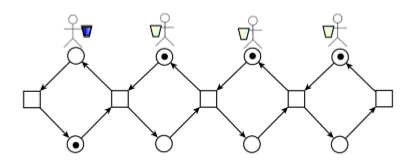
\includegraphics[width=0.7\textwidth]{img/reti/rete_spegnimento_fuoco.png}
    \caption{Esempio di una rete per modellare il sistema di spegnimento del fuoco}
    \label{fig:spegnimento-fuoco}
\end{figure}
\begin{definizione}[\textbf{Rete causale}]
    Definiamo $N = (B,E, F)$ come una \textbf{rete causale}, detta anche rete di
    occorrenze senza conflitti, se e solo se:
    \begin{itemize}
        \item $\forall b \in B: |^{\bullet}b| \leq 1 \land |b^{\bullet}| \leq 1$
              ovvero non si hanno conflitti; quindi, per ogni condizione si ha al più
              un pre-evento e un post evento. (Avendo quindi al più un arco entrante
              e al più uno uscente).
        \item $\forall x, y \in B \cup E: (x, y) \in F^{+} \Rightarrow (y, x) \notin F^{+})$
              ovvero non si hanno cicli; quindi, presi due elementi collegati da una
              sequenza di archi orientati, avendo un cammino tra i due elementi ($F^{+}$
              è la chiusura transitiva della relazione $F$) non ho anche un cammino
              opposto tra i due.
        \item $\forall e \in E: \{x \in B \cup E | xF^{\ast}e\}$ è finito, ovvero
              si ha un numero finito di pre-elementi di un certo elemento.
    \end{itemize}
    Sono quindi reti che registrano un comportamento e quindi non si hanno
    conflitti (che in caso sono sciolti registrando solo quello che è effettivamente
    successo e non quello che potrebbe succedere). Si registra una run del sistema.
    Non si hanno nemmeno cicli perché ogni ripetizione dell'evento viene concatenata
    a quella prima.

    La rete può quindi essere infinita, ma è composta da un insieme di elementi
    finito che si ripete. In ogni caso il passato di un evento è finito e registrato,
    anche se nel complesso il comportamento è infinito “in avanti”. Con una rete
    causale si possono non distinguere più condizioni ed eventi.
\end{definizione}
Ad una rete causale è possibile associare un \textbf{ordine parziale}:
\begin{equation}
    (X, \leq) = (B \cup E, F^{\ast})
\end{equation}
Dicendo che un elemento “è minore” di un altro se esiste un cammino orientato
dall'uno all'altro.
\begin{definizione}
    Data una rete causale $N = (B,E, F)$ e dato un ordine parziale $(X, \leq)$
    con $X = B \cup E$ si ha che si può interpretare la relazione d'ordine come
    indipendenza o dipendenza causale, ovvero presi $x, y \in X$ come elementi
    che occorrono nella storia di $X = B \cup E$ si hanno le seguenti diciture:
    \begin{itemize}
        \item $x \leq y$ (avendo un cammino da $x$ a $y$) corrisponde a $x$ causa
              $y$, ovvero si ha una relazione di dipendenza causale tra i due.
        \item $x \ \textbf{li} \ y$ indica che $x \leq y \lor y \leq x$ e quindi
              corrisponde a $x$ e $y$ sono causalmente dipendenti. Si ha che \textbf{li}
              può venire letto come linea ($x$ in linea con $y$) avendo che uno dei
              due precede l'altro.
        \item $x \textbf{co} \ y$ indica che: $\lnot(x < y)\  \land  \ \lnot (y < x)$
              e quindi corrisponde a $x$ e $y$ sono \textbf{causalmente indipendenti},
              avendo che i due elementi non si precedono a vicenda, non avendo ordine
              tra loro. Si ha che \textbf{co} sta per concurrency.
    \end{itemize}
    Le relazioni \textbf{li} e \textbf{co} sono riflessive e simmetriche ma non transitive.
\end{definizione}
\begin{definizione}
    Data una rete causale $N = (B,E, F)$ e dato un ordine parziale $(X, \leq)$
    con $X = B \cup E$ definiamo:
    \begin{equation}
        C \subseteq X
    \end{equation}
    come:
    \begin{itemize}
        \item \textbf{co-set} se e solo se $\forall x, y \in C$: $x \ \textbf{co} \ y$,
              quindi $C$ è una clique della relazione \textbf{co}.
        \item \textbf{taglio} se e solo se $C$ è un \textbf{co-set} massimale
              (tutti gli elementi nel taglio sono in relazione \textbf{co})
              \begin{equation}
                  \forall z\in X, \exists v\in C, z \ \textbf{li} \ v
              \end{equation}
    \end{itemize}
    Definiamo $C$ come \textbf{co-set} massimale se e solo se $\forall y \in X \cap C$
    si ha che:
    \begin{equation}
        \exists c \in C: y \not\textbf{co} \ c
    \end{equation}
    Quindi in $C$ definito o come \textbf{co-set} o come \textbf{taglio} si ha
    che \textbf{co} è transitività.

    Definiamo:
    \begin{equation}
        L \subseteq X
    \end{equation}
    come:
    \begin{itemize}
        \item \textbf{li-set} se e solo se $\forall x, y \in L: \ x \ \textbf{li} \ y$
        \item \textbf{linea} se e solo se $L$ è un \textbf{li-set} massimale.
              \begin{equation}
                  \forall z\in X, \exists v\in C, z \ \textbf{li} \ v
              \end{equation}
    \end{itemize}
    Definiamo $L$ come \textbf{li-set} massimale se e solo se $\forall y \in X
        \backslash L$ si ha che:
    \begin{equation}
        \exists l \in L: \ y \not\textbf{li}  \ l
    \end{equation}
    Si ha quindi che:
    \begin{itemize}
        \item In un \textbf{co-set} la relazione \textbf{co} è transitiva.
        \item In un \textbf{li-set} la relazione \textbf{li} è transitiva.
    \end{itemize}
    Tagli e linee possono essere fatti sia di condizioni che di eventi.
\end{definizione}
Un taglio $C \subseteq X$ è detto $B$-taglio se $C \subseteq B$.

I tagli fatti di sole condizioni rappresentano casi raggiungibili dal sistema.

Una rete causale, quindi, registra il comportamento di un sistema elementare. Si
hanno quindi, con i tagli, possibili osservazioni di configurazioni possibili
nella storia del sistema.
\begin{definizione}
    Grazie alle reti causali, preso un elemento $x \in X$, possiamo definire:
    \begin{itemize}
        \item $\textbf{past}(x)$, ovvero il passato dell'elemento, tutti gli
              elementi in relazione $\leq$ di $x$.
        \item $\textbf{future}(x)$, ovvero il futuro dell'elemento, tutti gli
              elementi in relazione $\geq$ di $x$.
    \end{itemize}
    Gli elementi nell'anti-cono sono in relazione \textbf{co} con $x$ e quindi
    possono essere concorrenti.
\end{definizione}
\begin{definizione}[\textbf{k-densità}]
    $N = (B, E, F)$ rete causale, $(X = (B \cup E), \leq)$ ordine parziale. Si
    ha che $N$ è \textbf{$k-$densa} se e solo se:
    \begin{equation}
        \forall h \in Linee(N), \ \forall c \in Tagli(N): \ |h \cap c| = 1
    \end{equation}
    dove $Linee(N)$ e $Tagli(N)$ sono gli insiemi delle linee e dei tagli di $N$.
\end{definizione}
\begin{nota}
    Se la rete causale $N$ è finita allora $N$ è anche $K-$densa.
\end{nota}
\begin{figure}[!ht]
    \centering
    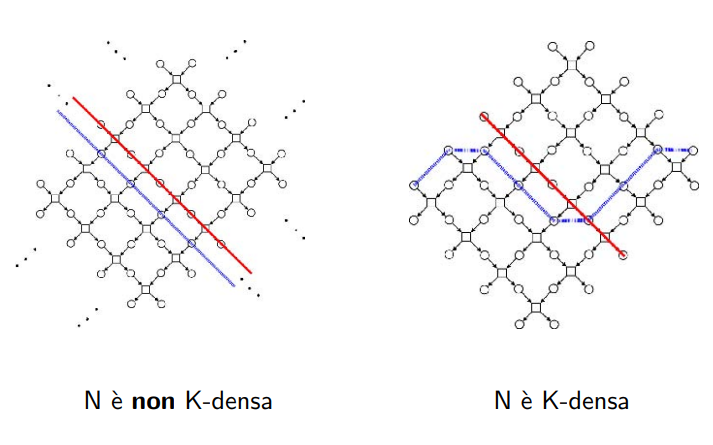
\includegraphics[width=0.7\textwidth]{img/reti/kdensa.png}
    \caption{Esempio di rete $K$-densa}
\end{figure}
\begin{definizione}[\textbf{Processi non sequenziali}]
    Sia $\Sigma = (S, T, F, c_{in})$ un sistema elementare senza contatti e finito,
    ovvero con $S \cup T$ finito.

    $\langle N = (B, E, F), \phi \rangle$ è un \textbf{processo non sequenziale}
    su $\Sigma$ se e solo se:
    \begin{itemize}
        \item $(B, E, F)$ è una rete causale nella quale si ammettono condizioni
              isolate.
        \item $\phi: B \cup E \to S \cup T$ è una mappa tale che:
              \begin{enumerate}
                  \item $\phi(B) \subseteq S, \ \phi(E) \subseteq T$
                  \item $\forall x_1, x_2 \in B \cup E: \ \phi(x_1) = \phi(x_2)
                            \Rightarrow (x_1 \leq x_2) \ \lor \ (x_2 \leq x_1)$
                  \item $\forall e \in E: \ \phi(^{\bullet}e) = ^{\bullet}\phi(e)
                            \ \land \ \phi(e^{\bullet}) = \phi(e)^{\bullet}$
                  \item $\phi(Min(N)) = c_{in}$ dove
                        $Min(N) = \{x \in B \cup E | \not\exists y: \ (y, x) \in F\}$
                        ovvero non hanno un arco entrante, sono gli stati locali
                        iniziali.
              \end{enumerate}
    \end{itemize}
\end{definizione}
Se $\langle N = (B, E, F); \phi \rangle$ è un processo non sequenziale di
$\Sigma = (S, T, F, c_{in})$ sistema elementare finito e senza contatti allora:
\begin{itemize}
    \item $N = (B, E, F)$ è $K$-densa
    \item $\forall K \subseteq B$, $K\ B$-taglio di $N$ è tale che: $K$ è finito e
          $\exists c \in C_{\Sigma}: \ \phi(K) = c$
\end{itemize}
I B-tagli corrispondono ai casi raggiungibili perché sono contemporaneamente veri.
\subsection{Reti di Occorrenze}
Vogliamo avere una struttura che registri tutti i comportamenti possibili
registrando le dipendenze e le indipendenze tra i processi. Posso avere una
struttura che mi raccolga tutti i possibili processi sequenziali.
\begin{definizione}[\textbf{Relazione di conflitto}]
    Una \textbf{relazione di conflitto}  $\#\subseteq (B\cup E)\times (B\cup E)$
    è definita come
    \begin{equation}
        x\#y\iff \exists e_1,e_2\in E :^{\bullet}e_1 \cap ^{\bullet} e_2\ne \emptyset
        \land e_1\le x \land e_2\le y
    \end{equation}
    due elementi sono in relazione se nel loro passato hanno 2 eventi in conflitto.
\end{definizione}
\begin{definizione}[\textbf{Rete di occorrenze}]
    $N = (B, E, F)$ è una \textbf{rete di occorrenze} se e solo se:
    \begin{itemize}
        \item \textbf{conflitti solo in avanti}: $\forall b \in B: \ | ^{\bullet}b|
                  \leq 1$ sono presenti dei conflitti solo in avanti.
        \item \textbf{aciclica}: $\forall x, y \in B \cup E: \ (x, y) \in F^{+}
                  \Rightarrow (y, x) \notin F^{+}$
              non ci sono cicli
        \item\textbf{passato finito}: $\forall e \in E: \{x \in B \cup E| \
                  xF^{\ast} e \}$ è finito
        \item \textbf{relazione di conflitto} $\#$ non è riflessiva.
    \end{itemize}
\end{definizione}
In queste reti è ancora possibile associare a $N$ un ordine parziale
$(X, \leq) = (B \cup E, F^{\ast})$. Se i due elementi non sono ordinati allora
saranno o in relazione $co$ o in \textbf{conflitto}. Estenderemo la relazione $co$
specificando $x\text{ co }y$ aggiunge il fatto che $\lnot x\#y$.
\begin{definizione}[\textbf{Processo ramificato}]
    Sia $\Sigma = (S,T, F, c_{in})$ un sistema elementare senza contatti e finito.
    $\langle N = (B, E, F); \phi \rangle$ è un \textbf{processo ramificato} di $\Sigma$
    se e solo se:
    \begin{itemize}
        \item $(B, E, F)$ è una rete di occorrenze (si ammettono condizioni isolate)
        \item $\phi: B \cup E \to S \cup T$ è una mappa:
              \begin{enumerate}
                  \item $\phi(B) \subseteq S, \ \phi(E) \subseteq T$
                  \item $\forall e_1, e_2 \in E: \ ( ^{\bullet} e_1 =  ^{\bullet}
                            e_2 \ \land \ \phi(e_1) = \phi(e_2)) \Rightarrow e_1 = e_2$
                  \item $\forall e \in E$ : la restrizione di $\phi$ a $^{\bullet} e$
                        è una biiezione tra $^{\bullet} e \ \text{e} \ ^{\bullet} \phi(e)$
                        e la restrizione di $\phi$ a $e^{\bullet}$ è una biiezione tra
                        $e^{\bullet} \ \text{e} \ \phi(e)^{\bullet}$
                  \item La restrizione di $\phi$ a $Min(N)$ è una biiezione tra
                        $Min(N)$ e $c_{in}$.
              \end{enumerate}
    \end{itemize}
\end{definizione}
La proprietà 2 e 3 delle reti causali in and tra loro implicano la proprietà 3
delle reti di occorrenze. Un ragionamento analogo può essere fatto per le proprietà
2 e 4 delle reti causali, le quali in and implicano la proprietà 4 delle reti
di occorrenza.
\begin{nota}
    Un processo non sequenziale può essere definito anche richiedendo che $\phi$
    soddisfi: (1),(2),(3') e (4'), dove 3' e 4' implicano le proprietà 3 e 4
    delle reti di occorrenza.
\end{nota}
\begin{definizione}[\textbf{Prefisso}]
    Sia $\Sigma = (S,T, F, c_{in})$ un sistema elementare finito e senza contatti
    e siano $\Pi_1 = \langle N_1; \phi_1 \rangle$, $\Pi_2 = \langle N_2; \phi_2 \rangle$
    processi ramificati di $\Sigma$.

    Allora $\Pi_1 = \langle N_1; \phi_1 \rangle$ è un \textbf{prefisso} di
    $\Pi_2 = \langle N_2; \phi_2 \rangle$ se e solo se $N_1$ è una sottorete di
    $N_2$ e $\phi_{2|N_1} = \phi_1$ ($\phi_2$ ”ristretto” a $N_1$ è uguale a $\phi_1$).
\end{definizione}
\begin{definizione}[\textbf{Unfolding}]
    $\Sigma$ ammette un unico processo ramificato che è massimale rispetto alla
    relazione di prefisso tra processi. Tale processo massimale è chiamato
    \textbf{unfolding} di $\Sigma$, denotato $Unf (\Sigma)$.
\end{definizione}
\begin{definizione}[\textbf{Corsa}]
    Un processo non sequenziale è un processo ramificato $\Pi = \langle N; \phi \rangle$
    tale che $N$ sia una rete causale (senza conflitti), tale processo è chiamato
    anche \textbf{corsa} (\textbf{run}).
\end{definizione}
\begin{osservazione}
    Inoltre, ogni processo non sequenziale di $\Sigma$ è un prefisso dell'unfolding
    $Unf (\Sigma)$.
\end{osservazione}
\section{Sistemi elementari - reti P/T- Reti ad alto livello}
Se dovessimo usare le reti elementari per modellare sistemi veri, avremmo
un'esplosione di condizioni ed eventi. Una rappresentazione più compatta è data
dalle \textbf{reti Posti e Transizioni} che utilizzano, invece delle condizioni
booleane dei sistemi elementari, dei contatori.
\begin{definizione}[\textbf{Sistema Posti e Transizioni}]
    Formalmente un sistema posti e transizioni è definito come:
    \begin{equation}
        \sigma = (S, T, F, K, W, M_0)
    \end{equation}
    dove:
    \begin{itemize}
        \item $(S, T, F)$ è una rete.
        \item $K: S \to \mathbb{N}^+ \cup \{\infty\}$ è la funzione che assegna ai
              posti le capacità
        \item $W: F \to \mathbb{N}$ è la funzione peso degli archi
        \item $M_0: S \to \mathbb{N}: \forall s \in S$ $M_0(s) \leq K(s)$ è la
              marcatura iniziale. È importante osservare che il numero di marche è sempre
              minore o uguale alla capacità del posto
    \end{itemize}
\end{definizione}
Ad esempio, pensiamo ad un buffer a due posizioni, nei sistemi elementari avremmo
due condizioni con due eventi deposita e preleva. Nei sistemi P/T possiamo usare
un contatore come fosse un'unica condizione. Chiaramente si perde dell'informazione,
in particolare non sappiamo più in quale posizione del buffer il produttore
deposita e da quale posizione il consumatore consuma.

Questa tipologia di reti mi permette di definire degli archi pesati, archi con
associato un numero, che abilitino o meno le transizioni.

Le reti ad alto livello, anche dette \textbf{reti colorate}, permettono di
ristabilire l'informazione persa con le reti Posti e transizioni assegnando una
struttura dati alle marche. Addirittura, una marca potrebbe rappresentare un
processo a sé stante.
\begin{definizione}[\textbf{Regola di scatto}]
    Sapendo che $M:S\to \mathbb{N}$ è la funzione che restituisce la marcatura di
    uno stato e $t\in T$ è un evento:
    \begin{equation}
        M[t > \ \text{se e solo se} \ \forall s \in S \ M(s) \geq W(s, t) \ \land
        \ M(s) \ + \ W(t, s) \leq K(s)
    \end{equation}
    \begin{equation}
        M[t > M' \ \text{se e solo se} \ M[t > \ \land \ \forall s \in S \ M'(s)
        = M(s) - W(s, t) + W(t, s)
    \end{equation}
\end{definizione}
\begin{definizione}
    $\Sigma = (S,T,F,K,W,M_0)$ un \textbf{sistema} $P/T$, l'insieme delle
    \textbf{marcature raggiungibili} di $\Sigma$ è $[M_0>$, il più piccolo
    insieme tale che:
    \begin{itemize}
        \item $M_0\in [M_0>$
        \item $M\in [M_0>\land \exists t\in T: M[t>M'\implies M' \in [M_0>$
    \end{itemize}
\end{definizione}
\begin{definizione}
    $\Sigma = (S,T,F,K,W;M_0)$ un \textbf{sistema} $P/T$ allora
    $RG(\Sigma)=([M_0>,U_\Sigma,A,M_0)$ è il \textbf{grafo di raggiungibilità}
    di $\Sigma$, dove
    \begin{equation}
        S=\left\{(M,U,M'):M,M'\in [M_0>\land U\in U_\Sigma\land M[U>M' \right\}
    \end{equation}
\end{definizione}
Anche qui, come nei sistemi elementari si può costruire l'insieme delle marcature
raggiungibili e il relativo grafo di raggiungibilità. Generalmente in queste reti
la Diamond property non è più valida, questo causa self-loop.

Come per i sistemi elementari, anche nelle reti a P/T è possibile aggiungere posti
per eliminare situazione di \textbf{contatto}, eliminando il vincolo sulla capacità,
senza alterare il comportamento del sistema. Questo si può fare mediante la
\textbf{complementazione} con stati.
\begin{definizione}
    Un sistema $P/T$ $\Sigma = (S,T,F,K,W;M_0)$ è \textbf{senza contatti} sse
    $\forall M\in [M_0>,\forall t\in T, \forall s\in S$:
    \begin{equation}
        M(s)\ge W(s,t)\implies M(s)+W(t,s)\le K(s)
    \end{equation}
\end{definizione}
Se $\Sigma = (S,T,F,K,W;M_0)$ è un \textbf{sistema} $P/T$ senza contatti allora
$t$ è \textbf{abilitata} in $M\in [M_0>$ ($M[t>$) sse
\begin{equation}
    \forall s\in S M(s)\ge W(s,t)
\end{equation}
Nei sistemi senza contatti la \textbf{capacità} non ha alcun ruolo nella regola
di scatto perché la transizione può scattare se nei suoi posti di input ci sono
abbastanza marche.
\begin{definizione}[\textbf{Reti marcate}]
    Un sistema Posti e transizione è una rete marcata se non ha vincoli sulla
    capacità dei posti e ha tutti gli archi di peso unitario.
    \begin{equation}
        \forall s\in S, M_0(s)\in \mathbb{N}\land K(s)=\infty \land \forall t\in
        T, W(s,t)\le 1\land W(t,s)\le 1
    \end{equation}
    Le reti marcate sono denotate da $(S,T,F;M_0)$ in quanto $K,W$ sono ridondanti
\end{definizione}

\begin{definizione} [\textbf{Reti marcate sicure}]
    $\Sigma = (S,T,F;M_0)$ una \textbf{rete marcata} allora è \textbf{sicura}
    (\textbf{safe}) sse:
    \begin{equation}
        \forall M\in [M_0>,\forall s\in S:M(s)\le1
    \end{equation}
\end{definizione}
Una rete marcata è \textbf{safe} se comunque evolva il comportamento avremmo in
ogni posto sempre al più una marca, i posti hanno quindi $0$ o $1$ marca e possiamo
interpretarli di nuovo come condizioni booleane. L'unica differenza con le reti
elementari è che nelle reti safe i cappi sono abilitati, mentre nelle reti
elementari questo non succede. Se eliminiamo i cappi dalle reti marcate safe,
otteniamo il corrispettivo di un sistema elementare puro.

\begin{definizione}
    Sia $\Sigma = (S,T,F,K,W;M_0)$ è un \textbf{sistema} $P/T$ tale che
    $\forall s\in S,K(s)=\infty$ e $N=(S,T,F)$ è \textbf{senza cappi}. Allora il
    sistema può essere rappresentato da un'unica matrice $\underline{N}:S\times
        T\rightarrow\mathbb{N}$
    chiamata \textbf{matrice di incidenza}.
\end{definizione}
Quindi avremo che
\begin{equation}
    M_0[t_1>\iff \underline{M_0}+\underline{t_1}\ge \underline{0} (\iff
    \underline{M_0}+\underline{N_{t_1}}\ge \underline{0})
\end{equation}
Quindi ogni cambio di stato lo possiamo codificare con una somma di vettori colonna,
utilizzando l'\textbf{equazione di stato}:
\begin{equation}
    M_0[\sigma>M_1\implies \underline{M_0}+\underline{N}\cdot \underline{c_\sigma}
    =\underline{M_1}
\end{equation}

\begin{osservazione}
    Sia $\Sigma = (S,T,F,K,W,M_0)$ un \textbf{sistema} $P/T$ tale che $\forall s
        \in S, K(s)=\infty$:
    \begin{itemize}
        \item $\Sigma$ è \textbf{limitato} sse $\exists n\in \mathbb{N}: \forall
                  s\in S, \forall M\in [M_0>$:
              $$M(s)\le n$$
        \item $\Sigma$ è \textbf{safe} sse $$\forall s\in S \forall M\in
                  [M_0>:M(s)\le 1$$
        \item
              $\Sigma$ è \textbf{limitato} $\iff [M_0>$ è un insieme \textbf{finito}
              ($RG(\Sigma)$ è \textbf{finito}).
        \item $\Sigma$ è \textbf{terminante} sse non ammette sequenze infinite
        \item $M\in [M_0>$ è una marcatura di \textbf{deadlock} sse $\forall t\in
                  T,\lnot(M[t>)$
        \item $\Sigma$ è \textbf{deadlock-free} sse $\forall M\in[M_0>\exists t\in
                  T:M[t>$
              $$(\iff \not\exists M\in [M_0>:M\text{ è una marcatura di deadlock})$$
        \item $\Sigma$ è $1$\textbf{-vivo} sse
              $$\forall t\in T,\exists M\in [M_0>:M[t>$$
        \item  $\Sigma$ è \textbf{vivo} sse
              $$\forall t\in T,\forall M\in [M_0>,\exists M'\in [M>:M'[t>$$
              \textbf{vivezza} $\implies$ assenza di \textbf{deadlock}.
        \item $\Sigma$ è \textbf{reversiblile} (ciclico) sse
              $$\forall M\in [M_0>:M_0\in [M>$$
        \item $\Sigma$ è \textbf{reversibile} $\iff$ il suo grafo delle marcature
              raggiungibili è \textbf{strettamente connesso}
        \item reversibilità $+ 1$-vivezza$\implies$ vivezza
    \end{itemize}
\end{osservazione}

Per verificare le proprietà allora si può fare:
\begin{itemize}
    \item analisi del grafo di raggiungibilità o di un prefisso dell'unfolding
    \item analisi strutturale del grafo della rete:
          \begin{itemize}
              \item tecniche che sfruttano l'algebra lineare come le \textbf{equazioni
                        di stato} che descrivono la dinamica e le $S$-invarianti
                    e le $T$-invarianti
              \item studio del grafo della rete come sottoinsiemi di nodi...
              \item controllo delle condizioni necessarie e sufficienti per alcune
                    sottoclassi di reti.
          \end{itemize}
\end{itemize}


\subsection{Reti ad alto livello}
Dal momento che le reti P/T hanno un problema di perdita di informazioni, allora
si può risolvere modellando le marche (contatori) con una struttura dati.